\chapter{Конструкторский раздел}
В этом разделе содержатся схемы алгоритмов поиска подстроки в строке и алгоритм поиска по словарю.
\section{Метод поиска по словарю при ограничении на значение признака, заданном при помощи лингвистической переменной}

Ниже приведены этапы метода поиска по словарю при ограничении на значение признака, заданном при помощи лингвистической переменной:
\begin{itemize}[label=---]
\item найти вхождение слова описывающего объект (например <<видео>>)
\item найти вхождение слов/словосочетаний указывающих на признак (например <<количество просмотров>>)
\item найти терм (например <<маленькое>>, <<очень маленькое>>, <<не очень маленькое>>, <<большое>> и так далее)
\item найти элементы словаря, удовлетворяющие значению терма.
\end{itemize}

Перевод термов в числовые значения осуществляются по наибольшему из значений функций $\mu_i(x_j)$ на конкретном значении из \eqref{eq:znach}.

\section{Разработка алгоритмов}

На рисунке \ref{fig:subsearch} представлена схема алгоритма поиска подстроки в строке.
\captionsetup{justification=centering,singlelinecheck=false}
\begin{figure}[H]
	\center{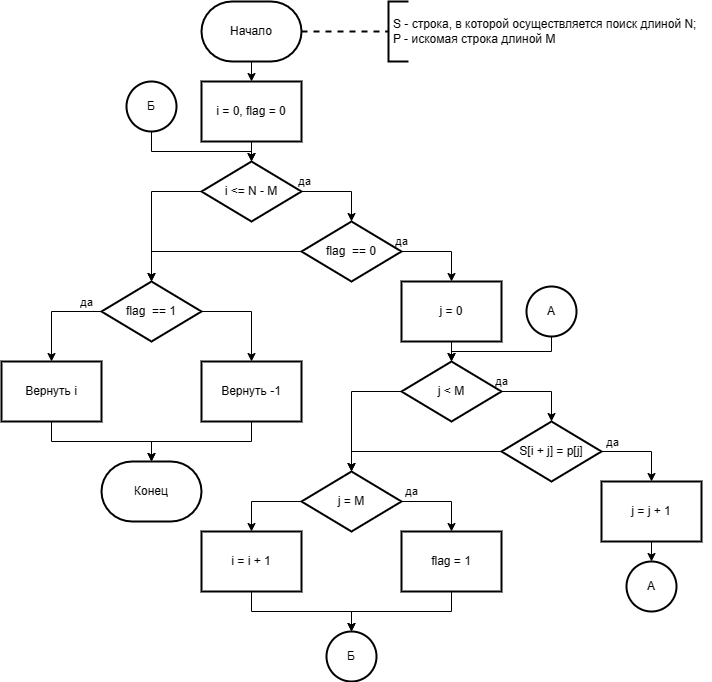
\includegraphics[scale=0.6]{inc/img/subsearch.png}}
	\caption{Cхема алгоритма поиска подстроки в строке}
	\label{fig:subsearch}
\end{figure}
\newpage

На рисунке \ref{fig:binary_search} представлен алгоритм полного перебора поиска по словарю. 
\begin{figure}[H]
	\center{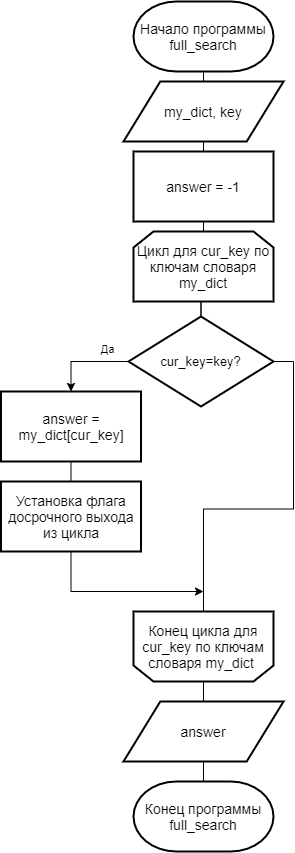
\includegraphics[scale=0.64]{inc/img/binary_search.png}}
	\caption{Схема алгоритма полного перебора для поиска по словарю}
	\label{fig:binary_search}
\end{figure}

\section*{Вывод}
В данном разделе были разработаны схема алгоритма поиска подстроки в строке и схема алгоритма полного перебора для поиска по словарю, описаны этапы метода поиска в словаре при ограничении на значение признака, заданном при помощи лингвистической переменной.

